\documentclass{beamer}

\usepackage{hyperref}
\usepackage{fancyhdr}
\usepackage{nameref}
\usepackage[symbol]{footmisc}
\usepackage{minitoc}
\usepackage{color}
\usepackage{amsmath}
\usepackage[francais]{babel}
\usepackage{natbib}
\usepackage{amssymb}
\usepackage[utf8]{inputenc}
\usepackage[footheight=1em]{beamerthemeboxes}
\usepackage{array}
\setcounter{tocdepth}{3}

\newcommand{\HRule}{\rule{\linewidth}{0.5mm}}
\renewcommand{\thefootnote}{\fnsymbol{footnote}}
\renewcommand{\contentsname}{Table des matières}

% Macros relatives à la traduction de PH avec arcs neutralisants vers PH à k-priorités fixes

% Macros générales
%\newcommand{\ie}{\textit{i.e.} }
\newcommand{\segm}[2]{\llbracket #1; #2 \rrbracket}
%\newcommand{\f}[1]{\mathsf{#1}}

% Notations générales pour PH
\newcommand{\PH}{\mathcal{PH}}
%\newcommand{\PHs}{\mathcal{S}}
\newcommand{\PHs}{\Sigma}
%\newcommand{\PHp}{\mathcal{P}}
\newcommand{\PHp}{\textcolor{red}{\mathcal{P}}}
%\newcommand{\PHproc}{\mathcal{P}}
\newcommand{\PHproc}{\mathbf{Proc}}
\newcommand{\Proc}{\PHproc}
\newcommand{\PHh}{\mathcal{H}}
\newcommand{\PHa}{\PHh}
%\newcommand{\PHa}{\mathcal{A}}
\newcommand{\PHl}{\mathcal{L}}
\newcommand{\PHn}{\mathcal{N}}
\newcommand{\PHt}{\mathcal{H}_{t}} % Ensemble des action du T-PH avec des actions temporisées

\newcommand{\PHhitter}{\mathsf{hitter}}
\newcommand{\PHtarget}{\mathsf{target}}
\newcommand{\PHbounce}{\mathsf{bounce}}
%\newcommand{\PHsort}{\Sigma}
\newcommand{\PHsort}{\PHs}
%State of PH
\newcommand{\PHst}{\zeta}

%Automata Network
\newcommand{\AN}{\mathcal{AAN}}
\newcommand{\TAN}{T-\mathcal{AN}}
\newcommand{\ANsort}{\Sigma}
\newcommand{\ANbound}[1]{\operatorname{b}(#1)}
\newcommand{\ANstate}{\mathcal{S}}
\newcommand{\ANtrans}{\mathcal{T}}
\newcommand{\ANst}{\zeta}
%\newcommand{\LS}{\textbf{LS}}
\newcommand{\LS}{\mathcal{LS}}
\newcommand{\ANgt}{\rightarrow}
\newcommand{\ANgtu}[1]{\ANgt_{#1}}
\newcommand{\origin}[1]{\mathsf{ori}(#1)}
\newcommand{\condition}[1]{\mathsf{cond}(#1)}
\newcommand{\destination}[1]{\mathsf{dest}(#1)}
%\newcommand{\ANuexp}[1]{U^{#1}}
\newcommand{\ANuexpsymbol}{\,\mathcal{U}}
\newcommand{\ANuexp}[1]{\ANuexpsymbol^{#1}}
\newcommand{\U}{\ANuexpsymbol}
\newcommand{\Ua}{\ANuexp{\mathsf{asyn}}}
\newcommand{\Us}{\ANuexp{\mathsf{syn}}}
\newcommand{\ANglobalstate}[1]{\langle #1 \rangle}
\newcommand{\ANltsymb}[4]{#1 \overset{#2}{#4} #3}
\newcommand{\ANlt}[3]{\ANltsymb{#1}{#2}{#3}{\rightarrow}}
\newcommand{\ANlts}[3]{\ANltsymb{#1}{\{#2\}}{#3}{\longrightarrow}}
\newcommand{\ANltsc}[3]{\textcolor{commentgray}{\ANlts{#1}{#2}{#3}}}
\newcommand{\aiellaj}{\ANlt{a_i}{\ell}{a_j}}
\newcommand{\trace}{\mathsf{trace}}
\newcommand{\successiverep}{\mathsf{sr}}

%\newcommand{\PHfrappeur}{\mathsf{frappeur}}
%\newcommand{\PHcible}{\mathsf{cible}}
%\newcommand{\PHbond}{\mathsf{bond}}
%\newcommand{\PHsorte}{\mathsf{sorte}}
%\newcommand{\PHbloquant}{\mathsf{bloquante}}
%\newcommand{\PHbloque}{\mathsf{bloquee}}

%\newcommand{\PHfrappeR}{\textcolor{red}{\rightarrow}}
%\newcommand{\PHmonte}{\textcolor{red}{\Rsh}}

\newcommand{\PHhitA}{\rightarrow}
\newcommand{\PHhitB}{\Rsh}
%\newcommand{\PHfrappe}[3]{\mbox{$#1\PHhitA#2\PHhitB#3$}}
%\newcommand{\PHfrappebond}[2]{\mbox{$#1\PHhitB#2$}}
\newcommand{\PHhit}[3]{#1\PHhitA#2\PHhitB#3}
\newcommand{\PHfrappe}{\PHhit}
\newcommand{\PHhbounce}[2]{#1\PHhitB#2}
\newcommand{\PHobj}[2]{\mbox{$#1\PHhitB^*\!#2$}}
\newcommand{\PHobjectif}{\PHobj}
\newcommand{\PHconcat}{::}
%\newcommand{\PHneutralise}{\rtimes}
\def\Sce{\mathbf{Sce}}

% Actions plurielles
\newcommand{\PHhitmultsymbol}{\rightarrowtail}
\newcommand{\PHhitmult}[2]{\mbox{$#1 \PHhitmultsymbol #2$}}
\newcommand{\PHfrappemult}{\PHhitmult}
\newcommand{\PHfrappemults}[2]{\PHhitmult{\{#1\}}{\{#2\}}}

%Action plurielle avec délai
\newcommand{\PHhitdelayB}{\Rsh}
\newcommand{\PHhitdelayA}[1]{\xrightarrow{#1} }
\newcommand{\PHhitdelay}[4]{#1\PHhitdelayA{#2} #3 \PHhitdelayB #4}
\newcommand{\PHfrappedelay}{\PHhitdelay}

\def\PHget#1#2{{#1[#2]}}
%\newcommand{\PHchange}[2]{#1\langle #2 \rangle}
%\newcommand{\PHchange}[2]{(#1 \Lleftarrow #2)}
%\newcommand{\PHarcn}[2]{\mbox{$#1\PHneutralise#2$}}
\newcommand{\PHplay}{\cdot}

\newcommand{\PHstate}[1]{\mbox{$\langle #1 \rangle$}}
\newcommand{\PHetat}{\PHstate}

\def\supp{\mathsf{support}}
\def\first{\mathsf{first}}
\def\last{\mathsf{last}}

\def\DNtrans{\rightarrow_{ADN}}
\def\DNdef{(\mathbb F, \langle f^1, \dots, f^n\rangle)}
\def\DNdep{\mathsf{dep}}
\def\PHPtrans{\rightarrow_{PH}}
\def\get#1#2{#1[{#2}]}
\def\encodeF#1{\mathbf{#1}}
\def\toPH{\encodeF{PH}}
\def\card#1{|#1|}
\def\decode#1{\llbracket#1\rrbracket}
\def\encode#1{\llparenthesis#1\rrparenthesis}
\def\Hits{\PHa}
\def\hit{\PHhit}
\def\play{\cdot}

\def\Pint{\textsc{PINT}}

\newcommand{\sN}{\mathbb{N}}

\input{macros/macros-ph}
\input{macros/tikzstyles2.tex}

\setbeamertemplate{footline}{
\leavevmode
\hbox{\hspace*{-0.06cm}
\begin{beamercolorbox}[wd=.2\paperwidth,ht=2.25ex,dp=1ex,center]{author in head/foot}
	\usebeamerfont{author in head/foot}\insertshortauthor  %~~(\insertshortinstitute)
\end{beamercolorbox}
\begin{beamercolorbox}[wd=.6\paperwidth,ht=2.25ex,dp=1ex,center]{section in head/foot}
	\usebeamerfont{section in head/foot}\insertshorttitle
\end{beamercolorbox}
\begin{beamercolorbox}[wd=.2\paperwidth,ht=2.25ex,dp=1ex,right]{section in head/foot}
	\usebeamerfont{section in head/foot}\hspace*{2em}
	\insertframenumber{} / \inserttotalframenumber\hspace*{2ex}
\end{beamercolorbox}}
\vskip0pt
}



\title{Analyse de la dynamique des modèles biologiques par programmation logique}
\author{Léo-Paul Delsaux}
\institute{Stage effectué au laboratoire CRIStAL de Villeneuve-d'Ascq}
\date{juin-août 2022}

% ceci est un commentaire
% pour compiler : tapez pdflatex ex-presentation
% regardez ensuite le fichier ex-presentation.pdf

\begin{document}

\maketitle

\begin{frame}{Introduction}
	Mots-clés :
	\begin{itemize}
		\item Bio-informatique
		\item Answer Set Programming (ASP)
		\item Réseau d'automates asynchrone (AAN)
		\item \'Etat local/global, transition locale/globale, chemin, cycle, automate produit, attracteur
	\end{itemize}
\end{frame}

\begin{frame}{ASP}
	\pause
	parent(moi, papa).\\
	\pause
	parent(papa, papi).\\
	\textcolor{white}{cheatcode}\\
	\pause
	$\Rightarrow$ grandparent(moi, papi).
\end{frame}

\begin{frame}{ASP - Règles}
	parent(moi, papa).\\
	parent(papa, papi).\\
	\textcolor{white}{cheatcode}\\
	\pause
	\textcolor{blue}{grandparent(moi, papi) :- parent(moi, papa), parent(papa, papi).}\\	
\end{frame}

\begin{frame}{ASP - Variables}
	parent(moi, papa).\\
	parent(papa, papi).\\
	\textcolor{white}{cheatcode}\\
	\pause
	\textcolor{blue}{grandparent(X, Z) :- parent(X, Y), parent(Y, Z).}\\
	\textcolor{white}{cheatcode}\\
	\pause
	$\Rightarrow$ \textcolor{blue}{grandparent(moi, moi) :- parent(moi, moi), parent(moi, moi).}\\
		      \textcolor{blue}{grandparent(moi, moi) :- parent(moi, papa), parent(papa, moi).}\\
		      \verb![...]! (24 lignes supplémentaires)\\
		      \textcolor{blue}{grandparent(papi, papi) :- parent(papi, papi), parent(papi, papi).}
\end{frame}

\begin{frame}{ASP - Agrégats et contraintes}
	parent(moi, papa).\\
	parent(papa, papi).\\
	\textcolor{white}{cheatcode}\\
	\pause
	\textcolor{blue}{famille(moi). famille(papa). famille(papi).}\\
	\pause	
	\textcolor{blue}{1 \{ grandparent(X, Y) :- famille(X), famille(Y) \} 1.}\\
	\pause
	\textcolor{white}{cheatcode}\\
	\textcolor{blue}{:- famille(X), famille(Y), famille(Z),\\
	\pause
	\textcolor{white}{cheatcode} not grandparent(X, Z), parent(X, Y), parent(Y, Z).}
\end{frame}

\begin{frame}{Hitori}
	\begin{figure}[!h]
		\includegraphics[width=6cm]{hitori.png}
		\caption{Grille de Hitori (\href{https://fr.wikipedia.org/wiki/Hitori}{https://fr.wikipedia.org/wiki/Hitori})}
		\label{label-figure1}
	\end{figure}
\end{frame}

\begin{frame}{Hitori résolu}
	\begin{figure}[!h]
		\includegraphics[width=6cm]{Hitori_2.png}
		\caption{Grille de Hitori résolu (\href{https://fr.wikipedia.org/wiki/Hitori}{https://fr.wikipedia.org/wiki/Hitori})}
		\label{label-figure2}
	\end{figure}
\end{frame}

\begin{frame}{Hitori - Règles}
	\textcolor{blue}{
	\pause
	size(5).\\
	\textcolor{white}{cheatcode}\\
	val(1..S) :- size(S).\\
	column(1..S) :- size(S).\\
	row(1..S) :- size(S).\\
	\textcolor{white}{cheatcode}\\
	\pause
	color(0;1).\\
	\textcolor{white}{cheatcode}\\
	\pause
	1 \{ s(R, C, V) : color(V) \} 1 :- column(C), row(R).}\\
\end{frame}

\begin{frame}{Hitori - Règles (suite)}
	\textcolor{blue}{:- s(R, C, 1), s(R+1, C, 1).\\
	:- s(R, C, 1), s(R-1, C, 1).\\
	:- s(R, C, 1), s(R, C+1, 1).\\
	:- s(R, C, 1), s(R, C-1, 1).\\
	\textcolor{white}{cheatcode}\\
	\pause
	:- s(R, C, 0), s(R, C2, 0), C != C2, c(R, C, V), c(R, C2, V).\\
	:- s(R, C, 0), s(R2, C, 0), R != R2, c(R, C, V), c(R2, C, V).\\
	\textcolor{white}{cheatcode}\\
	\pause
	chemin((R1, C1), (R2, C2)) :- chemin((R1, C1), (X, Y)), chemin((X, Y), (R2, C2)).\\
	chemin((R, C),(R+1, C)) :- s(R, C, 0), s(R+1, C, 0).\\
	chemin((R, C),(R-1, C)) :- s(R, C, 0), s(R-1, C, 0).\\
	chemin((R, C),(R, C+1)) :- s(R, C, 0), s(R, C+1, 0).\\
	chemin((R, C),(R, C-1)) :- s(R, C, 0), s(R, C-1, 0).\\
	:- s(R, C, 0), s(R2, C2, 0), not chemin((R, C), (R2, C2)).}\\
\end{frame}

\begin{frame}{Sokoban}
	\begin{figure}[!h]
		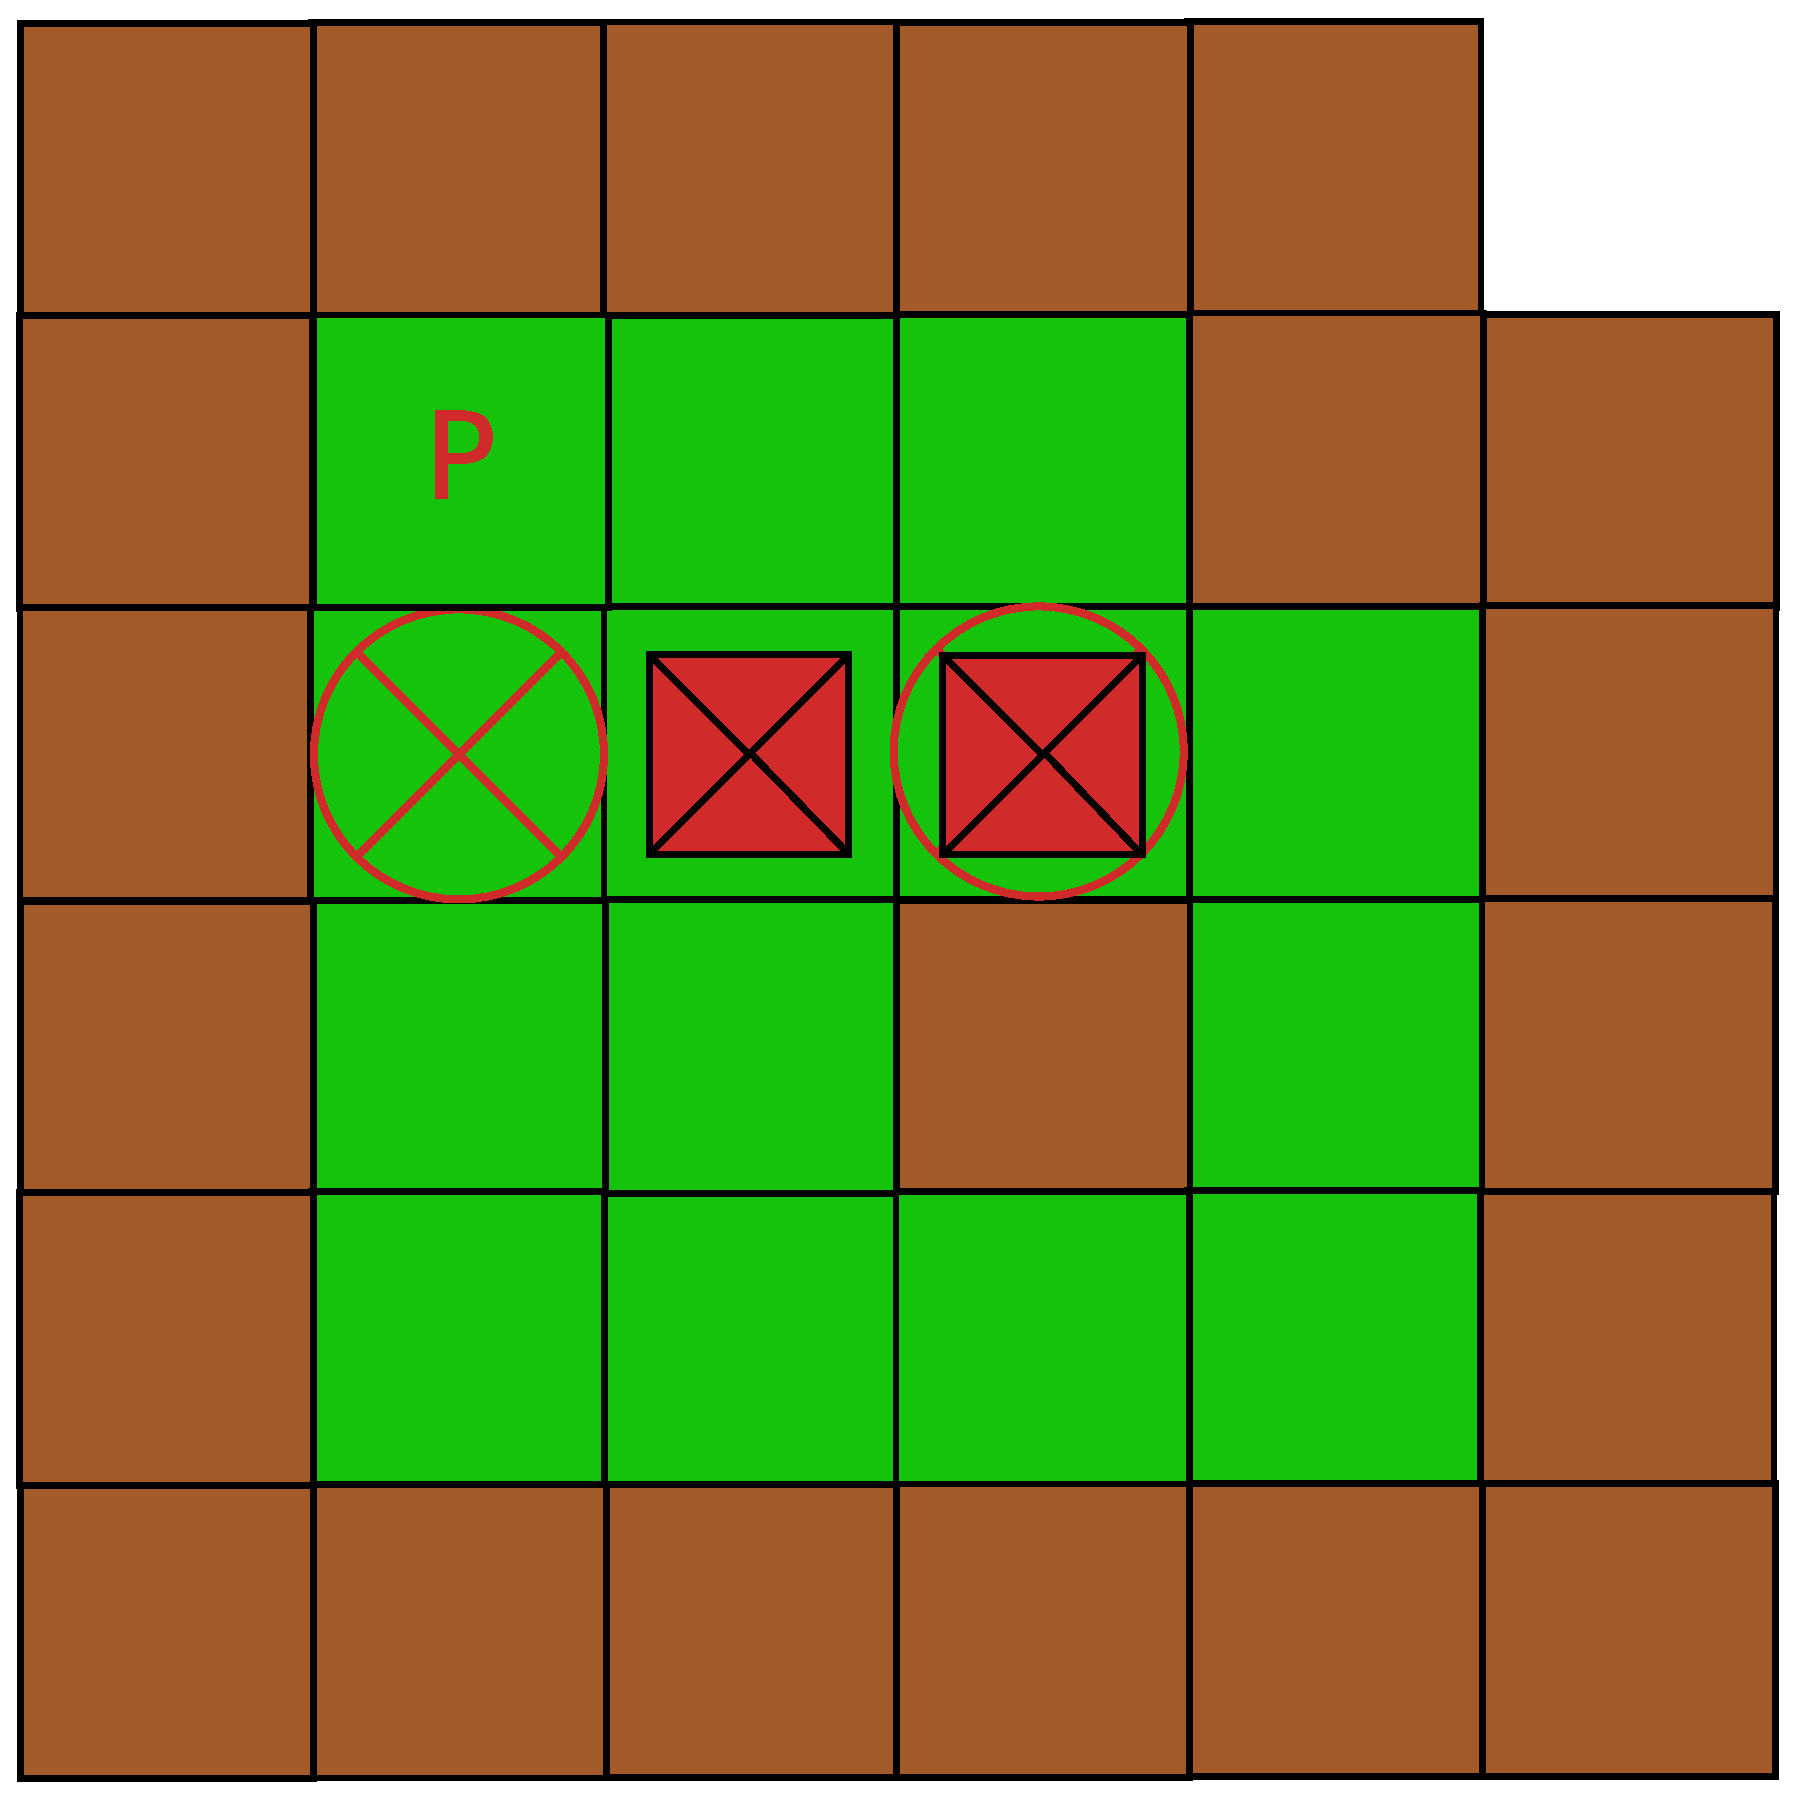
\includegraphics[width=6cm]{Diagram1.eps}
		\caption{Grille de Sokoban. P symbolise le joueur, les ronds rouges sont les cases d'arrivée, et les carrés rouges représentent les caisses.}
		\label{label-figure3}
	\end{figure}
\end{frame}

\begin{frame}{Sokoban - Stratégies de calcul}
	\begin{itemize}
		\item Naïf : on considère un coup en tant que déplacement possible du personnage
		\pause
		\item Plus rapide : on ne considère que les coups de déplacement de caisse. On considère alors un ensemble connexe de cases atteignables depuis celles du personnage
		\pause
		\item Autres améliorations mineures :
		\begin{itemize}
			\item Si une caisse est bloquée dans un coin sans arrivée, on arrête la recherche courante
			\item Si deux caisses sont dans un couloir (cernées par des murs), on arrête la recherche courante
			\item etc...
		\end{itemize}
	\end{itemize}
\end{frame}

\begin{frame}{AAN - Formalismes}
	Un réseau d'automates asynchrone est un triplet $(\Sigma,S,T)$, avec :
	\begin{itemize}
		\pause
		\item $\Sigma=\left\{a,b,...\right\}$ est un ensemble fini d'automates non vides.
		\pause
		\item Si $C_a$ est le nombre d'états d'un automate $a$, alors $S_a=\left\{a_0,a_1,...,a_{C_a-1}\right\}$ est l'ensemble des \textbf{états locaux} de $a$. $S=\displaystyle{\prod_{a\in\Sigma}}S_a$ est 
		l'ensemble fini des \textbf{états globaux}, et $LS=\displaystyle{\bigcup_{a\in\Sigma}}S_a$ représente l'ensemble de tous les états locaux.
		\pause
		\item Pour chaque $a\in\Sigma$, $T_a\subseteq\left\{a_i\xrightarrow{l}a_j\in S_a\times\rho(LS/S_a)\times S_a|a_i\neq a_j\right\}$ est l'ensemble des \textbf{transitions locales} d'un automate $a$, avec 
		$\rho$ qui désigne la puissance ensembliste. $T=\displaystyle{\bigcup_{a\in\Sigma}}T_a$ est l'ensemble des transitions locales du modèle.
	\end{itemize}
\end{frame}

\begin{frame}{AAN - Exemple}
	On prend l'AAN suivant comme exemple de référence pour ce qui suit : 
	\begin{itemize}
		\pause
		\item $\Sigma =\left\{a,b,c\right\}$
		\pause
		\item $S_a=\left\{a_0,a_1,a_2\right\}$, $S_b=\left\{b_0,b_1\right\}$ et $S_c=\left\{c_0,c_1,c_2\right\}$
		\pause
		\item $T_a = \left\{a_0\xrightarrow{b_0}a_1,a_0\xrightarrow{b_1,c_1}a_1,a_1\xrightarrow{b_1}a_0,a_1\xrightarrow{b_0}a_2,a_2\xrightarrow{b_1}a_1\right\}$\\
		$T_b=\left\{b_0\xrightarrow{c_0}b_1,b_1\xrightarrow{a_2}b_0\right\}$\\
		$T_c=\left\{c_0\xrightarrow{b_1}c_1,c_0\xrightarrow{a_2}c_2,c_1\xrightarrow{b_0}c_0,c_1\xrightarrow{a_1}c_2,c_2\xrightarrow{b_1}c_0\right\}$
	\end{itemize}
\end{frame}

\begin{frame}{AAN - Schéma de l'exemple}
	\begin{figure}[!h]
		\centering  
		\begin{tikzpicture}[apdotsimple/.style={apdot}]
		  \TSort{(0,2)}{a}{3}{r}
		  \TSort{(2.5,0)}{b}{2}{r}
		  \TSort{(5,2)}{c}{3}{r}

		  \path[local transitions]
		    (a_0) edge node[auto] {$b_0$} (a_1)
		    (a_1) edge node[auto] {$b_0$} (a_2)
		    (a_2) edge node[auto] {$b_1$} (a_1)
		    (a_1) edge node[auto] {$b_1$} (a_0)

		    (b_0) edge node[auto] {$c_0$} (b_1)
		    (b_1) edge node[auto] {$a_2$} (b_0)

		    (c_0) edge node[auto] {$b_1$} (c_1)
		    (c_1) edge node[auto] {$b_0$} (c_0)
		    (c_1) edge node[auto] {$a_1$} (c_2)
		    ;
		  \path[local transitions, bend left = 105]
		      (a_0) edge node[auto] {$b_1, c_1$} (a_1)
		    ;
		  \path[local transitions, bend left = 90]
		      (c_0) edge node[auto] {$a_2$} (c_2)
		    ;
		  \path[local transitions, bend left = 90]
		      (c_2) edge node[auto] {$b_1$} (c_0)
		    ;

		  \TState{a_0, b_1, c_1}
		\end{tikzpicture}
		
		\caption{Schéma de notre exemple de référence}
		\label{label-figure4}
	\end{figure}
\end{frame}

\begin{frame}{AAN - Traduction de l'exemple en ASP}
	En ASP, on définit l'exemple de référence en deux temps.\\
	\begin{itemize}
		\pause
		\item On déclare les niveaux : \\
			\textcolor{blue}{
			automaton\_level("a", 0..2).\\
			automaton\_level("b", 0..1).\\
			automaton\_level("c", 0..2).\\
			}
		\pause
		\item Et les transitions à l'aide de label : \\
			\textcolor{blue}{
			condition(t1, "a", 0). target(t1, "a", 1). condition(t1, "b", 0).\\
			condition(t2, "a", 1). target(t2, "a", 2). condition(t2, "b", 0).}\\
			\verb![...]!(11 lignes supplémentaires)\\
			\textcolor{blue}{condition(t12, "a", 0). target(t12, "a", 1). condition(t12, "b", 1). condition(t12, "c", 1).\\
			}
	\end{itemize}
\end{frame}

\begin{frame}{Sémantiques}
	On s'intéressera à 3 sémantiques principalement : 
	\begin{itemize}
		\pause
		\item asynchrone : les transitions globales sont exactement les transitions locales jouables
		\pause
		\item synchrone : les transitions globales sont les ensembles de transitions locales jouables de cardinal maximal (on doit jouer une transition locale pour chaque automate quand c'est psosible)
		\pause
		\item générale : les transitions globales sont générés par les parties de l'ensemble des transitions globales de la sémantique synchrone (on peut jouer une transition locale pour un automate, mais il faut qu'on en 
		joue au moins une)
	\end{itemize}
\end{frame}

\begin{frame}{Attracteurs}
	\pause
	Un \textbf{domaine de piège} est un ensemble d'états globaux duquel toutes les transitions globales pour la sémantique choisie mène à un élément de ce domaine.\\
	\pause
	Un \textbf{attracteur} est un domaine de piège minimal en terme d'inclusion ensembliste.\\
	\pause
	\textcolor{white}{cheatcode}\\
	\textbf{Lemme :} Les attracteurs d'un AAN sont exactement les domaines de piège cycliques.
\end{frame}

\begin{frame}{Cœur de la contribution personnelle}
	\pause
	Solutions étudiées : 
	\begin{itemize}
		\pause
		\item correction de la troisième contrainte en Python
		\pause
		\item utilisation des états globaux en ASP
	\end{itemize}
\end{frame}

\begin{frame}{Correction de la troisième contrainte en Python}
	\pause
	Une fois que l'on a généré tous les chemins possibles dans un AAN à l'aide d'agrégats, il nous faut filtrer les ensembles-solutions qui nous intéressent. On doit alors respecter 3 contraintes : \\
	\begin{itemize}
		\pause
		\item avoir un cycle
		\pause
		\item tout les états globaux du chemin visités après l'étape de fin du visite du cycle doivent être des éléments de ce dernier
		\pause
		\item toutes les transitions globales jouables depuis chacun des éléments du cycle doivent arriver dans un autre élément de ce cycle ( = domaine piège)\\
	\end{itemize}
\end{frame}

\begin{frame}{Correction de la troisième contrainte en Python - Résultats}
	\begin{figure}[!h]
		\begin{tabular}{l|c<{\onslide<2->}c<{\onslide<3->}c<{\onslide<4->}c<{\onslide<5->}c<{\onslide<6->}c<{\onslide<7->}c<{\onslide}c}
			n & exam. & lamb. & trp. & fis. & mamm. & tcr. & t-helper \\ \hline
			2     & 2 & 2 & 0 & 1 & 0 & 0 & 8878\\
			5     & 2 & 2 & 1 & 1 & 0 & 0 & 5477\\
			10    & 2 & 2 & 1 & 1 & 1 & 1 & 4072\\
			15    & 2 & 2 & 1 & 1 & 1 & 1 & 2850
		\end{tabular}
		\caption{Nombre d'attracteurs trouvés pour la sémantique synchrone (version avec python)}
		\label{label-figure5}
	\end{figure}
	
	\begin{figure}[!h]
		\begin{tabular}{l|c<{\onslide<2->}c<{\onslide<3->}c<{\onslide<4->}c<{\onslide<5->}c<{\onslide<6->}c<{\onslide<7->}c<{\onslide}c}
			n & exam. & lamb. & trp. & fis. & mamm. & tcr. & t-helper \\ \hline
			2     & .051 & .053 & .044 & .047 & .047 & .049 & T.O\\
			5     & .052 & .060 & .039 & .057 & .043 & .079 & T.O\\
			10    & .054 & .076 & .050 & .084 & .082 & .201 & T.O\\
			15    & .093 & .096 & .051 & .108 & .123 & .362 & T.O
		\end{tabular}
		\caption{Temps (en s) de résolution pour la sémantique synchrone (version avec python)}
		\label{label-figure5}
	\end{figure}
\end{frame}

\begin{frame}{Seconde solution : travail sur les états globaux - Résultats}
	\pause
	Une autre manière de gérer la troisième contrainte consiste à créer des prédicats pour les états globaux, et de mémoriser dans la sémantique quels sont les coups jouables depuis un état global, et non une étape temporelle 	
	donnée.\\
	
\end{frame}

\begin{frame}{Seconde solution : travail sur les états globaux - Résultats}
	\begin{figure}[!h]
		\begin{tabular}{l|c<{\onslide<2->}c<{\onslide<3->}c<{\onslide}c}
			n & exam. & lamb. & trp.\\ \hline
			2     & 2 & 2 & 0\\
			5     & 2 & 2 & 1\\
			10    & 2 &  & 1\\
		\end{tabular}
		\caption{Nombre d'attracteurs trouvés pour la sémantique synchrone (version avec états globaux)}
		\label{label-figure5}
	\end{figure}
	
	\begin{figure}[!h]
		\begin{tabular}{l|c<{\onslide<2->}c<{\onslide<3->}c<{\onslide}c}
			n & exam. & lamb. & trp.\\ \hline
			2     & 3.943 & 40.267 & 4.004\\
			5     & 5.435 & 58.742 & 5.461\\
			10    & 9.790 & T.O & 9.965\\
		\end{tabular}
		\caption{Temps (en s) de résolution pour la sémantique synchrone (version avec états globaux)}
		\label{label-figure5}
	\end{figure}
	REFAIRE LES BONS TESTS !!!
\end{frame}

\begin{frame}{Conclusions et pistes}
	\begin{itemize}
		\pause
		\item 2 versions fonctionnelles dont une peu efficace
		\pause
		\item La seconde version pourrait être améliorée avec de l'incrémental
		\pause
		\item Considérer des classes d'équivalence des attracteurs, et manipuler des sortes de "bassins d'attraction"
		\pause
		\item Combiner les deux idées précédentes (?)
	\end{itemize}
\end{frame}

\begin{frame}{Remerciements}
	Merci à :
	\begin{itemize}
		\item l'ENS de Lyon qui m'a proposé ce stage
		\item Maxime Folschette pour son encadrement
		\item les personnes au sein de l'équipe BioComputing
		\item mes quelques collègues stagiaires de bureau
		\item les auditeurs présents dans cette salle pour leur écoute
	\end{itemize}
\end{frame}

\end{document}



